We know that, since $Y = (X+1)^2$, 
\begin{align}
F_Y(y) = 0 \; \forall \; y < 0
\end{align}
Therefore, for $y\geq 0$, 
\begin{align}
F_Y(y) &= \pr{(x+1)^2 \leq y} \\
&= \pr{-\sqrt{y} - 1 \leq x \leq \sqrt{y} - 1 } \\
&= \pr{-\sqrt{y} - 1 \leq x \leq \sqrt{y} - 1 } \\
&= F_X(\sqrt{y} - 1) - F_X(-\sqrt{y} - 1) 
\label{st/2019/43/eqn_}
\end{align}
Since $X$ is a uniform random variable in $(-1, 1)$,
\begin{align}
f_X(x) &= 
\begin{cases}
\frac{1}{2} & -1 < x < 1 \\
0 & \text{otherwise}
\end{cases}\\
F_X(x) &= 
\begin{cases}
0 & x \leq -1 \\
\frac{x}{2} + \frac{1}{2} & -1 < x < 1 \\
1 & x \geq 1
\end{cases}
\label{st/2019/43/cdf_x}
\end{align}
Using \eqref{st/2019/43/cdf_x} in \eqref{st/2019/43/eqn_}, and using the fact that 
\begin{align}
-\sqrt{y}-1 \leq -1 \; \forall \; y \geq 0,
\end{align}
we get
\begin{align}
F_Y(y) &=  \begin{cases}
F_X(\sqrt{y} - 1) - 0 & y \geq 0\\
0 & y < 0
\end{cases} \\
&= \begin{cases}
0 & y < 0 \\
\frac{\sqrt{y}}{2}  & 0 \leq y \leq 4\\
1 & y > 4
\end{cases}
\end{align}
Therefore, 
\begin{align}
f_Y(y) &= \begin{cases}
\frac{1}{4\sqrt{y}}  & 0 \leq y \leq 4\\
0 & \text{otherwise}
\end{cases}
\end{align}
Therefore, \textbf{option 2} is correct. Fig. \ref{st/2019/43/CDF_Y} shows a theoretical vs simulated plot of the PDF of random variable $Y$.
\begin{figure}[!hbt]
    \centering
	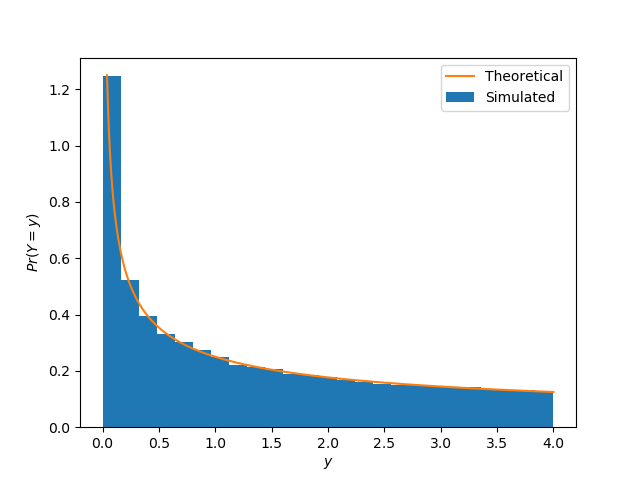
\includegraphics[width=\columnwidth]{solutions/adv/st/2019/43/Figures/Figure_1.png}
    \caption{The PDF of $Y$}
    \label{st/2019/43/CDF_Y}
\end{figure}
